\section{Hiện thực backend}

\subsection{Môi trường phát triển và công nghệ sử dụng}
\begin{itemize}
    \item Ngôn ngữ: Python 3.10+.

    \item Framework: FastAPI (đảm bảo hiệu năng cao, hỗ trợ Asynchronous).
    
    \item Database: PostgreSQL 15+ kết hợp với PostGIS (xử lý tọa độ bản đồ) và pgvector (xử lý Vector AI).
    
    \item ORM: SQLAlchemy 2.0 (quản lý truy vấn thông qua Model).
    
    \item Migration: Alembic (quản lý lịch sử thay đổi cấu trúc Database).
    
    \item Môi trường: Docker \& Docker-compose (để đóng gói và triển khai nhanh).
\end{itemize}

\subsection{Cấu trúc thư mục dự án}

Để đảm bảo tính linh hoạt, dễ bảo trì và khả năng mở rộng, mã nguồn của hệ thống Backend được tổ chức theo kiến trúc phân lớp (Layered Architecture). Cấu trúc thư mục chi tiết của dự án được trình bày như sau:

\begin{mycode}[Project Directory Structure]{}
uniconnect/
    app/
        api/                # API Layer (Routes)
            v1/             # API Version 1
                api.py      # Main router entry point
                endpoints/  # Specific endpoint logic (auth, activity, etc.)
        core/               # Core configurations (config, security)
        crud/               # Basic CRUD operations
        models/             # SQLAlchemy model definitions (ERD mapping)
        schemas/            # Pydantic schemas (Data Validation)
        services/           # Business logic layer (RAG, AI processing)
        db/                 # Database session management
        main.py             # Application entry point
    alembic/                # Database migrations management
    tests/                  # Automated test cases
    .env                    # Environment variables
    docker-compose.yml      # Container orchestration config
    Dockerfile              # Container image definition
    requirements.txt        # Python project dependencies
\end{mycode}

\subsection{Mô tả các thành phần hệ thống}
Việc tổ chức mã nguồn theo cấu trúc trên giúp tách biệt rõ ràng giữa logic nghiệp vụ, giao diện lập trình và truy xuất dữ liệu. Các thành phần chính bao gồm:

\begin{itemize}
    \item \textbf{Thư mục \texttt{app/models/}:} Hiện thực hóa sơ đồ ERD thành các lớp Python thông qua SQLAlchemy ORM. Tại đây, các ràng buộc dữ liệu, khóa chính, khóa ngoại và các kiểu dữ liệu đặc thù như \textit{Geography} (cho bản đồ) và \textit{Vector} (cho AI) được định nghĩa chặt chẽ.
    
    \item \textbf{Thư mục \texttt{app/api/}:} Đóng vai trò lớp biên (Boundary), định nghĩa các Endpoint để Frontend tương tác. Cách tiếp cận này giúp hệ thống có khả năng nâng cấp các phiên bản API độc lập mà không gây ảnh hưởng đến các thành phần cũ.
    
    \item \textbf{Thư mục \texttt{app/services/}:} Đây là lớp chứa đựng logic nghiệp vụ chính. Các xử lý phức tạp như: quy trình tìm kiếm ngữ nghĩa RAG, tính toán không gian bản đồ, hay logic phê duyệt người dùng tham gia hoạt động được tập trung tại đây để tối ưu hóa việc tái sử dụng mã nguồn.
    
    \item \textbf{Thư mục \texttt{app/schemas/}:} Sử dụng thư viện Pydantic để định nghĩa các cấu trúc dữ liệu trao đổi (DTO). Lớp này đảm bảo mọi dữ liệu đầu vào và đầu ra đều được kiểm tra kiểu dữ liệu (Validation) nghiêm ngặt trước khi xử lý.
    
    \item \textbf{Hệ thống \texttt{alembic/}:} Đảm nhận vai trò quản lý các phiên bản cấu trúc cơ sở dữ liệu. Mọi thay đổi trong mô hình dữ liệu đều được ghi vết và cập nhật đồng bộ vào Database thực tế thông qua các kịch bản Migration, đảm bảo tính toàn vẹn dữ liệu.
    
    \item \textbf{Docker và Containerization:} Toàn bộ hệ thống Backend và các dịch vụ bổ trợ (PostgreSQL, pgvector) được đóng gói trong các Container riêng biệt, giúp đồng nhất môi trường phát triển và môi trường vận hành thực tế.
\end{itemize}

\subsection{Hiện thực các tính năng cốt lõi}

\subsubsection{Xử lý dữ liệu không gian và Bản đồ (Geospatial Handling)}
Để quản lý các hoạt động trên bản đồ campus, hệ thống sử dụng tiện ích mở rộng \textit{PostGIS} của PostgreSQL kết hợp với thư viện \textit{GeoAlchemy2}. Dữ liệu tọa độ được lưu trữ dưới định dạng hình học \texttt{POINT} với hệ tọa độ \texttt{SRID 4326}.

\begin{mycode}[Geospatial Field Definition in Activity Model]{Python}
# Define geospatial Point field (latitude, longitude)
location = Column(Geography(geometry_type='POINT', srid=4326), nullable=True)

@property
def latitude(self):
    """Extract latitude from Geometry data"""
    if self.location is not None:
        return to_shape(self.location).y
    return None

@property
def longitude(self):
    """Extract longitude from Geometry data"""
    if self.location is not None:
        return to_shape(self.location).x
    return None
\end{mycode}

Việc hiện thực này cho phép hệ thống thực hiện các truy vấn không gian phức tạp như tìm kiếm các hoạt động trong bán kính nhất định xung quanh người dùng với hiệu năng tối ưu.

\subsubsection{Hệ thống tìm kiếm ngữ nghĩa và Trợ lý AI (RAG)}
Đây là tính năng trọng tâm của dự án, cho phép người dùng hỏi đáp dựa trên kho học liệu nội bộ. Hệ thống thực hiện quy trình RAG qua các bước:
\begin{enumerate}[leftmargin=*]
    \item \textbf{Vector hóa:} Sử dụng mô hình Embedding (như Sentence-Transformers hoặc Gemini) để chuyển đổi nội dung tài liệu thành các Vector 768 chiều.
    \item \textbf{Lưu trữ:} Sử dụng tiện ích \textit{pgvector} để lưu trữ và lập chỉ mục (Index) các Vector này.
    \item \textbf{Truy xuất:} Sử dụng toán tử khoảng cách Cosine (\textit{Cosine Similarity}) để tìm kiếm các đoạn văn bản có ý nghĩa gần nhất với câu hỏi của người dùng.
\end{enumerate}

\begin{mycode}[Vector Similarity Search Query]{SQL}
-- Find the top 5 chunks with similarity > 0.7
-- The <=> operator calculates Cosine Distance
-- Subtract from 1 to obtain Cosine Similarity
SELECT 
    content, 
    1 - (embedding <=> '[vector_query]') AS similarity
FROM resources
WHERE 1 - (embedding <=> '[vector_query]') > 0.7
ORDER BY similarity DESC 
LIMIT 5;
\end{mycode}

\subsubsection{Authentication}

Hệ thống triển khai cơ chế xác thực dựa trên tiêu chuẩn JSON Web Token (JWT). Mật khẩu người dùng được mã hóa bằng thuật toán bcrypt nhằm đảm bảo an toàn dữ liệu. Khi đăng nhập thành công, hệ thống cấp một mã định danh (Access Token) để người dùng thực hiện các yêu cầu tiếp theo thông qua lớp trung gian (Middleware).

\begin{mycode}[JWT and Password Security]{Python}
from jose import jwt
from passlib.context import CryptContext
from datetime import datetime, timedelta
Security configuration
pwd_context = CryptContext(schemes=["bcrypt"], deprecated="auto")
SECRET_KEY = "your_secret_key"
ALGORITHM = "HS256"

def create_access_token(data: dict):
"""Generate JWT for authenticated users"""
to_encode = data.copy()
expire = datetime.utcnow() + timedelta(minutes=30)
to_encode.update({"exp": expire})
return jwt.encode(to_encode, SECRET_KEY, algorithm=ALGORITHM)

def get_password_hash(password):
"""Hash password using bcrypt"""
return pwd_context.hash(password)
\end{mycode}

\subsubsection{Interactive API Documentation (Swagger UI)}

Một trong những ưu điểm cốt lõi của việc sử dụng FastAPI là khả năng tự động khởi tạo tài liệu API tương tác thông qua Swagger UI. Điều này giúp các nhà phát triển (đặc biệt là đội ngũ Frontend) dễ dàng theo dõi và thử nghiệm API mà không cần truy cập trực tiếp vào mã nguồn.

\begin{itemize}[leftmargin=*]
\item \textbf{Khám phá Điểm cuối (Endpoints):} Tất cả các đường dẫn (routes) được định nghĩa trong thư mục \texttt{app/api/v1/endpoints/} đều được chỉ mục hóa tự động.
\item \textbf{Kiểm soát dữ liệu đầu vào:} Giao diện hiển thị rõ ràng các lược đồ dữ liệu (Schemas) cần thiết cho mỗi yêu cầu, giúp giảm thiểu lỗi định dạng dữ liệu khi trao đổi giữa Client và Server.
\item \textbf{Thử nghiệm trực tiếp:} Cho phép thực hiện các yêu cầu HTTP (GET, POST, PUT, DELETE) trực tiếp trên trình duyệt để kiểm tra logic xử lý của Backend ngay lập tức.
\end{itemize}

\begin{figure}[H]
    \centering
    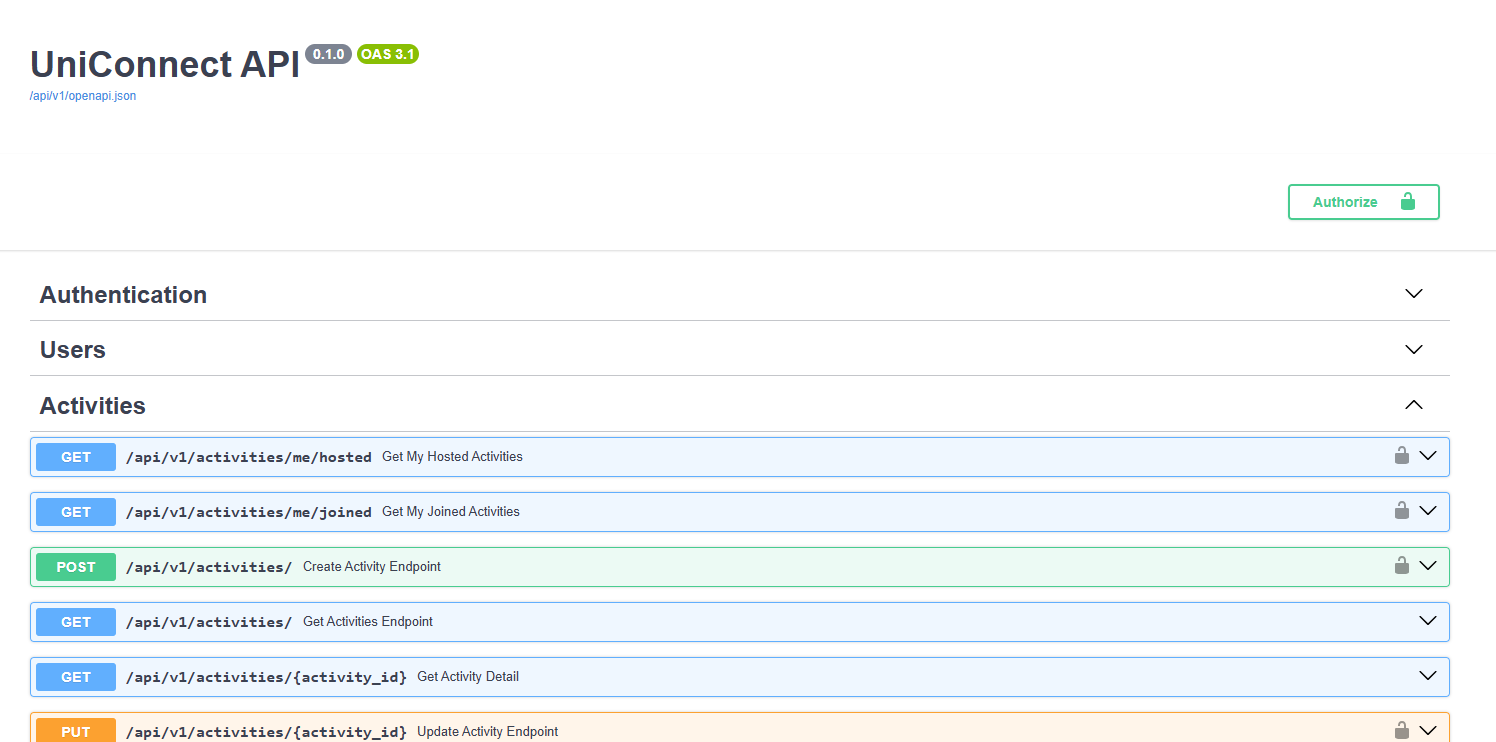
\includegraphics[width=0.85\textwidth]{Images/swagger.png} 
    \caption{Swagger UI của đề tài}
    \label{fig:swagger}
\end{figure}

\subsubsection{Đóng gói ứng dụng với Docker}

Để đảm bảo hệ thống vận hành ổn định trên mọi môi trường, dự án được đóng gói bằng công nghệ Docker. Toàn bộ dịch vụ bao gồm mã nguồn Backend và cơ sở dữ liệu PostgreSQL (tích hợp PostGIS/pgvector) được điều phối thông qua tệp cấu hình \texttt{docker-compose.yml}.

\begin{mycode}[Docker-Compose Orchestration]{}
services:
  # 1. Server Backend
  backend:
    build: .
    container_name: uniconnect_api
    ports:
      - "8000:8000"
    env_file:
      - .env
    volumes:
      - .:/app
    depends_on:
      db:
        condition: service_healthy
      redis:
        condition: service_started

  # 2. Database (Đã tích hợp PostGIS + pgvector)
  db:
    build: 
      context: .
      dockerfile: Dockerfile.db
    container_name: uniconnect_db
    environment:
      - POSTGRES_USER=\${DB_USER}
      - POSTGRES_PASSWORD=\${DB_PASSWORD}
      - POSTGRES_DB=\${DB_NAME}
    ports:
      - "5432:5432"
    volumes:
      - postgres_data:/var/lib/postgresql/data
    healthcheck:
      test: ["CMD-SHELL", "pg_isready -U \${DB_USER} -d \${DB_NAME}"]
      interval: 5s   
      timeout: 5s   
      retries: 5
      
  # 3. Redis
  redis:
    image: redis:alpine
    container_name: uniconnect_redis
    ports:
      - "6379:6379" 
    volumes:
      - redis_data:/data

volumes:
  postgres_data:
  redis_data:
\end{mycode}

Việc sử dụng Docker giúp rút ngắn thời gian triển khai và đảm bảo các thành phần mở rộng của cơ sở dữ liệu luôn sẵn sàng mà không cần cài đặt thủ công.

\subsection{Kết luận chương}

Chương này đã khái quát quá trình hiện thực hóa các thành phần cốt lõi của Backend, từ cấu trúc tổ chức mã nguồn đến các tính năng then chốt về xử lý dữ liệu không gian, tìm kiếm ngữ nghĩa và triển khai hệ thống. Đây là nền tảng vững chắc để phát triển giao diện người dùng và tích hợp các dịch vụ thông minh trong giai đoạn tiếp theo.

